\section{Nutzen des Algorithmus an Beispielen} % (fold)
\label{sec:PermutationExamples}
Aus der Vorlesung von Herrn Stroetmann und dem begleitenden Skript \autocite{github-stroetmann:online} ist bekannt, dass sich das Puzzle aus Abb. \ref{fig:Ex1_start} lösen, also in den Zielzustand aus Abb. \ref{fig:Ex1_end} überführen lässt.\\
\begin{minipage}{\linewidth}
	\begin{minipage}[t]{0.45\linewidth}
		\begin{figure}[H]
			\centering
			\includegraphics[width=\linewidth,keepaspectratio]{img/Ex1_start.png}
			\captionsetup{format=plain, indention=0pt}
			\caption{Beispiel1: Startzustand eines 4x4-Puzzles nach figure 2.20 aus \autocite{github-stroetmann:online} \label{fig:Ex1_start}}
		\end{figure}
	\end{minipage}
	\hfill
	\begin{minipage}[t]{0.45\linewidth}
		\begin{figure}[H]
			\centering
			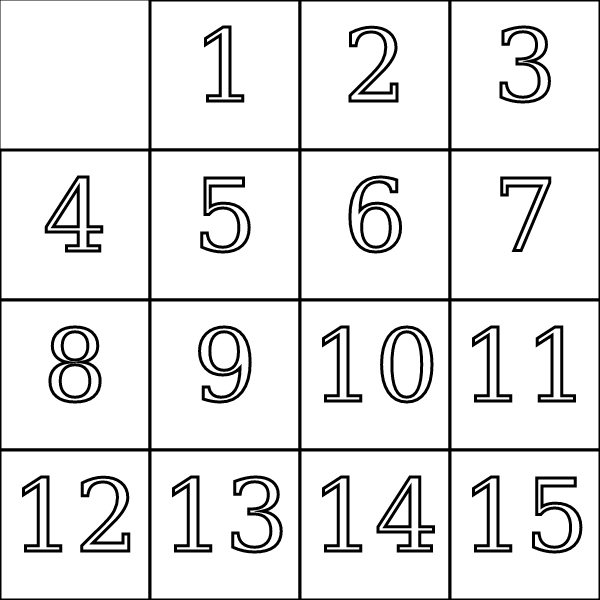
\includegraphics[width=\linewidth,keepaspectratio]{img/End_Puzzle_Stroetmann.png}
			\captionsetup{format=plain, indention=0pt}
			\caption{\label{fig:Ex1_end}Beispiel1: Zu erreichender Zielzustand für das Puzzle nach figure 2.20 aus \autocite{github-stroetmann:online}}
		\end{figure}
	\end{minipage}
\end{minipage}\\\WNL%
Der Algorithmus aus dem vorherigen Abschnitt schätzt diese Puzzles ebenfalls als lösbar ein.\\
\begin{figure}[H]
	\begin{enumerate}
		\item[\textbf{S1.1}] Konvertierung der Puzzle-Zustände in Zahlenreihen
		      \begin{align*}
			      start_{ex1} = \{0,1,2,3,4,5,6,8,14,7,11,10,9,15,12,13\} \\
			      end_{ex1} = \{0,1,2,3,4,5,6,7,8,9,10,11,12,13,14,15\}
		      \end{align*}
		\item[\textbf{S1.2}] Notwendige Transpositionen $T_{ex1}$ um $start_{ex1}$ zu sortieren:
		      \begin{align*}
			      0,1,2,3,4,5,6,8,14,7,11,10,9,15,12,13 & \hspace{20pt} (\space 8,\space 7) \\
			      0,1,2,3,4,5,6,7,14,8,11,10,9,15,12,13 & \hspace{20pt} (14,\space 8)       \\
			      0,1,2,3,4,5,6,7,8,14,11,10,9,15,12,13 & \hspace{20pt} (14,\space 9)       \\
			      0,1,2,3,4,5,6,7,8,9,11,10,14,15,12,13 & \hspace{20pt} (11,10)             \\
			      0,1,2,3,4,5,6,7,8,9,10,11,14,15,12,13 & \hspace{20pt} (14,12)             \\
			      0,1,2,3,4,5,6,7,8,9,10,11,12,15,14,13 & \hspace{20pt} (15,13)             \\
			      0,1,2,3,4,5,6,7,8,9,10,11,12,13,14,15 &
		      \end{align*}
		      \begin{align*}
			      T_{ex1} = \{(8,7),(14,8),(14,9),(11,10),(14,12),(15,13)\} \\
			      \left\vert T_{ex1}\right\vert = 6 \rightarrow \texttt{Parität} = 0
		      \end{align*}
		\item[\textbf{S1.3}] Anzahl der notwendigen Züge $z_{ex1}$ um das Leerfeld von der Postion aus dem Startzustand (Koordinaten $(0,0)$) an die Postion des Zielzustandes (Koordinaten $(0,0)$) zu verschieben.
		      \begin{align*}
			      z_{ex1} = \left | 0 - 0 \right | + \left | 0 - 0 \right | \\
			      z_{ex1} = 0 \rightarrow \texttt{Parität} = 0
		      \end{align*}
		\item[\textbf{S1.4}] Die Paritäten stimmen überein, das Puzzle \textcolor{OliveGreen}{ist lösbar}.
	\end{enumerate}
	\caption{Beispiel 1: Anwendung des Algorithmus auf ein Vorlesungsbeispiel \label{fig:Ex1_algo}}
\end{figure}
Dazu wird wie in Abb. \ref{fig:Ex1_algo} schrittweise vorgegangen. Zunächst werden, wie im Abschnitt \ref{sec:PuzzleToList} und in Schritt 1 (S1.1) dargestellt, die Zustände in Zahlenreihen konvertiert.
Anschließend werden die Paritäten ermittelt (S1.2 und S1.3). Zunächst die Parität der Anzahl notwendiger Transpositionen und anschlie"send die Parität benötigter Züge um die Leerstelle korrekt zu platzieren. Im abschlie"senden Schritt (S1.4) werden die ermittelten Paritäten verglichen. In diesem Beispiel stimmen diese Paritäten überein. Das Beispiel ist also lösbar.%
\WNL%
%
% Loyd
%
Als nächstes wird das Puzzle von Loyd aus der Einleitung betrachtet. Der bereits bekannte Startzustand ist in Abb. \ref{fig:Ex2_start} zur Vereinfachung erneut abgebildet. Der Zielzustand ist daneben in Abb. \ref{fig:Ex2_end} dargestellt.\\
\begin{minipage}{\linewidth}
	\begin{minipage}[t]{0.45\linewidth}
		\begin{figure}[H]
			\centering
			\includegraphics[width=\linewidth,keepaspectratio]{img/Ex2_start.png}
			\captionsetup{format=plain, indention=0pt}
			\caption{Beispiel2: Startzustand für das Loyd Puzzle \label{fig:Ex2_start}}
		\end{figure}
	\end{minipage}
	\hfill
	\begin{minipage}[t]{0.45\linewidth}
		\begin{figure}[H]
			\centering
			\includegraphics[width=\linewidth,keepaspectratio]{img/Ex2_end.png}
			\captionsetup{format=plain, indention=0pt}
			\caption{\label{fig:Ex2_end}Beispiel2: Zu erreichender Zielzustand für das Loyd Puzzle}
		\end{figure}
	\end{minipage}
\end{minipage}\\\WNL%
Auch hier wird der beschriebene Algorithmus angewandt, das Vorgehen ist in Abb. \ref{fig:Ex2_algo} skizziert.
\begin{figure}[H]
	\begin{enumerate}
		\item[\textbf{S2.1}] Konvertierung der Puzzle-Zustände in Zahlenreihen
		      \begin{align*}
			      start_{ex2} = \{1,2,3,4,5,6,7,8,9,10,11,12,13,15,14,0\} \\
			      end_{ex2} = \{1,2,3,4,5,6,7,8,9,10,11,12,13,14,15,0\}
		      \end{align*}
		\item[\textbf{S2.2}] Notwendige Transpositionen $T_{ex2}$ um $start_{ex2}$ zu $end_{ex2}$ zu überführen:
		      \begin{align*}
			      1,2,3,4,5,6,7,8,9,10,11,12,13,15,14,0 & \hspace{20pt} (15,14) \\
			      1,2,3,4,5,6,7,8,9,10,11,12,13,14,15,0 &
		      \end{align*}
		      \begin{align*}
			      T_{ex2} = \{(14,15)\} \\
			      \left\vert T_{ex2}\right\vert = 1 \rightarrow \texttt{Parität} = 1
		      \end{align*}
		\item[\textbf{S2.3}] Anzahl der notwendigen Züge $z_{ex2}$, um das Leerfeld von der Postion aus dem Startzustand (Koordinaten $(3,3)$) an die Postion des Zielzustandes (Koordinaten $(3,3)$) zu verschieben.
		      \begin{align*}
			      z_{ex1} = \left | 3 - 3 \right | + \left | 3 - 3 \right | \\
			      z_{ex1} = 0 \rightarrow \texttt{Parität} = 0
		      \end{align*}
		\item[\textbf{S2.4}] Die Paritäten stimmen nicht überein, das Puzzle ist somit \textcolor{red}{nicht lösbar}.
	\end{enumerate}
	\caption{Beispiel2: Anwendung des Algorithmus auf das Loyd Puzzle \label{fig:Ex2_algo}}
\end{figure}
Da die Zielzustände der beiden Puzzle verschieden sind (Abb. \ref{fig:Ex1_end} und Abb. \ref{fig:Ex2_end}), unterscheiden sich auch die Zahlenreihen als welche diese dargestellt werden. Doch zur Übersichtlichkeit wurde sowohl in S1.1 als auch in S2.1 die Leerstelle mit der Zahl \afz{0} kodiert. Es ist leicht zu erkennen, dass nur eine Transposition notwendig ist, um die Zahlenreihe $start_{ex2}$ in die Reihe $end_{ex2}$ zu überführen, die Parität des Vorgangs ist also 1. Da sich die Leerstelle bereits an der korrekten Stelle befindet, sind keine Züge notwendig, die Parität ist also 0. Da die Paritäten unterschiedlich sind, kategorisiert der Algorithmus dieses Puzzle korrekterweise als  nicht lösbar ein.\WNL
%
% endzustände
%
Die Wahl des Endzustandes ist relevant bei der Lösbarkeitsüberprüfung eines Puzzles. In der Sektion \ref{sec:Permutation} wurde explizit hervorgehoben, dass sich der in der Literatur übliche Endzustand (Abb. \ref{fig:Ex2_end}) von dem in Herrn Stroetmanns Skript \autocite{github-stroetmann:online} (Abb. \ref{fig:Ex1_end}) unterscheidet. In Abb. \ref{fig:Ex3_algo} zeigt der Algorithmus, dass diese Endzustände nicht ineinander Überführbar sind, In Schritt S3.1 werden Leerstellen erneut mit der Zahl \afz{0} kodiert.
\begin{figure}[H]
	\begin{enumerate}
		\item[\textbf{S3.1}] Konvertierung der Puzzle-Zustände in Zahlenreihen
		      \begin{align*}
			      end_{Loyd} = \{1,2,3,4,5,6,7,8,9,10,11,12,13,14,15,0\} \\
			      end_{Stroetmann} = \{0,1,2,3,4,5,6,7,8,9,10,11,12,13,14,15\}
		      \end{align*}
		\item[\textbf{S3.2}] Notwendige Transpositionen $T_{ex3}$ um $end_{Loyd}$ zu $end_{Stroetmann}$ überführen:
		      \begin{align*}
			      1,2,3,4,5,6,7,8,9,10,11,12,13,14,15,0 & \hspace{20pt} (1,0)   \\
			      0,2,3,4,5,6,7,8,9,10,11,12,13,14,15,1 & \hspace{20pt} (2,1)   \\
			      0,1,3,4,5,6,7,8,9,10,11,12,13,14,15,2 & \hspace{20pt} (3,2)   \\
			      0,1,2,4,5,6,7,8,9,10,11,12,13,14,15,3 & \hspace{20pt} (4,3)   \\
			      0,1,2,3,5,6,7,8,9,10,11,12,13,14,15,4 & \hspace{20pt} (5,4)   \\
			      0,1,2,3,4,6,7,8,9,10,11,12,13,14,15,5 & \hspace{20pt} (6,5)   \\
			      0,1,2,3,4,5,7,8,9,10,11,12,13,14,15,6 & \hspace{20pt} (7,6)   \\
			      0,1,2,3,4,5,6,8,9,10,11,12,13,14,15,7 & \hspace{20pt} (8,7)   \\
			      0,1,2,3,4,5,6,7,9,10,11,12,13,14,15,8 & \hspace{20pt} (9,8)   \\
			      0,1,2,3,4,5,6,7,8,10,11,12,13,14,15,9 & \hspace{20pt} (10,9)  \\
			      0,1,2,3,4,5,6,7,8,9,11,12,13,14,15,10 & \hspace{20pt} (11,10) \\
			      0,1,2,3,4,5,6,7,8,9,10,12,13,14,15,11 & \hspace{20pt} (12,11) \\
			      0,1,2,3,4,5,6,7,8,9,10,11,13,14,15,12 & \hspace{20pt} (13,12) \\
			      0,1,2,3,4,5,6,7,8,9,10,11,12,14,15,13 & \hspace{20pt} (14,13) \\
			      0,1,2,3,4,5,6,7,8,9,10,11,12,13,15,14 & \hspace{20pt} (15,14) \\
			      0,1,2,3,4,5,6,7,8,9,10,11,12,13,14,15
		      \end{align*}
		      \begin{align*}
			      T_{ex3} = \{(1,0),(2,1),(3,2),(4,3),(5,4),(6,5),(7,6),(8,7),(9,8),(10,9),(11,10), \\(12,11),(13,12),(14,13),(15,14)\}\\
		      \end{align*}
		      \begin{align*}
			      \left\vert T_{ex3}\right\vert = 15 \rightarrow \texttt{Parität} = 1
		      \end{align*}
		\item[\textbf{S3.3}] Anzahl der notwendigen Züge $z_{ex2}$ um das Leerfeld von der Postion aus Loyds Endzustand (Koordinaten $(3,3)$) an die Postion des Zielzustandes von Stroetmann (Koordinaten $(0,0)$) zu verschieben.
		      \begin{align*}
			      z_{ex3} = \left | 3 - 0 \right | + \left | 3 - 0 \right | \\
			      z_{ex3} = 6 \rightarrow \texttt{Parität} = 0
		      \end{align*}
		\item[\textbf{S3.4}] Die Paritäten stimmen nicht überein, das Puzzle ist somit \textcolor{red}{nicht lösbar}.
	\end{enumerate}
	\caption{Beispiel 2: Anwendung des Algorithmus auf die Überführbarkeit der Endzustände von Loyd und Stroetmann. \label{fig:Ex3_algo}}
\end{figure}
Ist ein Puzzle also für den einen Endzustand lösbar, ist es für den anderen Endzustand automatisch nicht lösbar, da es keine Möglichkeit gibt die Endzustände ineinander zu überführen.
%Endzustände

